\documentclass[msc, deptreport, ai, romanprepages]{infthesis}
\usepackage{times} %% This makes the body base font times...
\usepackage{url}
\usepackage{graphics}
\usepackage{graphicx}
\usepackage{amsmath, amsthm}
\usepackage{amssymb}
\usepackage{textcomp}
\usepackage[olditem]{paralist}
\usepackage{epsfig}
\usepackage{geometry}
\usepackage{indentfirst}
\usepackage{color} %May be necessary if you want to color links
\usepackage{hyperref}
\hypersetup{
colorlinks=false, %set true if you want colored links
linktoc=all, %set to all if you want both sections and subsections linked
}



\newcommand*{\defeq}{\stackrel{\text{def}}{=}}

\setlength{\parindent}{1.5em}
\setlength{\parskip}{1em}


\setcounter{tocdepth}{2}


\begin{document}

\title{Monte Carlo Planning in the Belief Domain to Play Cluedo}

\author{Joseph Ledford}

\course{Master of Artificial Intelligence}
\project{{\bf Dissertation}}

\date{\today}

\abstract{ This dissertation is concerned with creating an agent capable of playing the partially observable board game Cluedo by planning in the belief domain using Monte Carlo methods. We implemented a simulator that allows play between agents and optionally human players. This work is inspired by two recent methods for tractable learning in large complex partially observable games where we reason about our belief of the current game state rather than a fully observable state. We also analyze the strength of our main agent against a heuristic baseline.}

\maketitle

\section*{Acknowledgements}
Acknowledgements go here. 

\tableofcontents

\chapter{introduction}
The following paragraphs are based on the work done in my IPP report \cite{IPP}. The development of novel AI agents is accelerated when implemented in tandem with simulated environments where those agents and algorithms can explore in a consequence free manner. In comparison, testing with robotics in real environments can be slow and more importantly costly. Time ticks at a constant rate in the real world and cannot be sped up arbitrarily like learning done in a simulated environment. We also prefer to avoid the incurrence of any costs related to the consequences of failed attempts which necessarily follow from the learning process. Therefore games are appealing for reinforcement learning for their fast and cheap properties. They also allow measurements of incremental progress in the form of a score (many times simply win/lose), giving researchers comparable benchmarks. Many real world parallels are easily drawn to the activities and objectives of games, such as negotiation, collaborating to obtain resources, and strategical decisions. Games are designed implicitly from human experience, and naturally follow from decision-making problems found in the real world. Thus, it is easy to see why advancements made in game agents naturally extend to real-world planning. Games of imperfect information are particularly similar, at least conceptually, to real-world problems, where reasoning under uncertainty is necessary. Humans are often required to act in a world that they are implicitly uncertain about (therefore their actions may have unforeseen consequences). Similarly, these games are relevant because humans and agents often must act with reference to opponents or collaborators, whose goals, preferences and strategies they may not fully understand. 

Motivated by the above, this dissertation is concerned with the implementation of a simulator for the complex board game Cluedo, and the creation of a baseline heuristic based agent and a more theoretically informed reinforcement learning agent. This latter agent is an extension/adaptation to the work done by (Silver and Veness, 2010) and (Dobre, 2018) \cite{Silver-veness} \cite{Mihai}. This agent will plan in the belief domain and attempt to take advantage of the aspects of partial observability in the game. The doctoral thesis of Mihai Dobre is the inspiration for this work and as such, this dissertation is heavily influenced by his hypotheses and findings \cite{Mihai}. As a result, the motivation, structure and methods of this dissertation are analogous to those outlined by Dobre \cite{Mihai}. 

Cluedo is an interesting game for this dissertation because of its’ complexity and diverse attributes. It has a large state space, involves multi-agent play and has dominant aspects of imperfect information. The imperfect information lies in the uncertainty of opponents’ hands, the cards in the envelope and other players’ falsifications (which card they showed). The rewards are also highly sparse, meaning that the first and only reward signal is only observed when the game terminates. Thus, the sequence of states and actions from any state until an agent observes this signal (the end of the game) can be very long. This means that game trajectories represented as a tree have considerable depth. The game is sequential in nature (players take turns), symmetric (all agents are focused on the same goal) and non-cooperative. By far, the most important aspect of the game, and the one we are most interested in, is the partial observability. It is crucial to pay heed to the actions of others. Agents can continuously gather knowledge by reasoning about other players’ moves. In fact, humans play this game by implicitly reasoning about opponents’ actions. Any agent that fails to take advantage of this facet of the game will perform poorly. This is because, the questions asked by other agents and the corresponding cards shown (or also not shown) to them by a particular agent, can inform us as to the hands of other players. Cluedo however, is not continuous nor does it feature simultaneous actions, which is characteristic of real-life planning domains. In spite of this, its other defining characteristics are indeed worthwhile to explore and this makes Cluedo a valuable stepping stone in the field of sequential decision-making research.

\section{Hypothesis}
\begin{description}
\item \textbf{Emergent Structure Hypothesis (ESH):} There is a structure that arises naturally in highly complex games and it can be exploited to aid the learning process; 
\item \textbf{Model-based Abstraction Hypothesis (MAH):} One can use a model of the environment to reduce the complexity and improve the performance of the learning agent.
\end{description}

\section{Code}
The relevant code for all work done in this dissertation is available from the two following Java repositories:
\begin{description}
\item \textbf{Cluedo\_Sim:} https://github.com/jcl240/Cluedo\_Sim. This project contains all the code for the baseline/heuristic agents and the Cluedo simulator itself (with GUI). 
\item \textbf{MCTS:} https://github.com/sorinMD/MCTS. This project by Mihai Dobre contains the parallelized MCTS code used by the MCTS agent (with our own factored belief and state representation implemented, see appendices A and B)
\end{description}

\section{Limitations}
The principal aim of this thesis was to evaluate planning in the belief space for Cluedo. Due to time constraints the Monte Carlo agent presented in this dissertation has not been comprehensively optimized, nor were we able to focus our efforts on finding optimal hyperparameters. As a consequence, the aforementioned agent could be improved tenfold in terms of efficiency and performance. Thus, the results presented here are most likely indicative of a lower performance bound rather than a tight one from above and below. Further optimizations are left for future research and will most likely lead to increased performance. Due to our use of Heuristic opponents in the rollout phase of the MCTS algorithm, we introduce an implicit dependence between our MCTS agent and the strength of the heuristic agent. Better heuristics than the ones explored here (and they undoubtedly do exist) would also lead to increased performance. We limited our resources for planning to four cores, eight threads and a maximum of three and a half seconds of planning per decision. This was for the sake of time conservation and also to get a good idea of how the agent performs under circumstances tolerable by a human opponent on a reasonably powerful machine. 

\chapter{Background}
\section{Reinforcement Learning}
The following sections are based on the field survey of Reinforcement Learning in my IPP report \cite{IPP}. Reinforcement Learning is a field of machine learning which is concerned with the analysis and development of algorithms for sequential decision making problems. The distinct goal of RL is to choose actions sequentially so as to maximize/minimize a future objective (such as winning in a game or minimizing energy costs). The decisions made by reinforcement learning algorithms during simulated trajectories or an actual game are referred to aggregately as a policy. The policy followed during simulated trajectories, or rollouts, is specifically named the rollout policy. The objective is not to find any random policy, but rather compute the policy which maximizes future reward in an informed manner. In games of full observability and perfect information, like Go or Chess, there exists some optimal value function which determines that game when played optimally by all players (Silver et al., 2016) \cite{Silver2016}. In game theory this is known as a Nash equilibrium. However, this is not readily or obviously extendable to complex partially observable games like Cluedo or Settlers of Catan. Even if it was, an exhaustive search of all sequences to compute a Nash Equilibrium is not computationally feasible. Instead we look for algorithms that approximate the quality of an action ‘online’ in any given state encountered. Online meaning computing the action values as states are encountered. 

\section{Monte Carlo Tree Search}
Monte-Carlo Tree Search (MCTS) is the premier online quality estimator, which estimates via sampling full sequences of the game through self-play and averaging them together (Gelly et al., 2012) \cite{Gelly}. By performing rollouts (full simulations of the game from the current state), we build a tree which will eventually contain the optimal value estimates. Thus, MCTS has a very useful property: consistency. Given enough time, this sampling algorithm will find the optimal values for all nodes of the tree and can therefore select the optimal action at the root state \cite{Gelly}. MCTS slowly builds the game tree by using a core concept in RL, bootstrapping. By using the statistics from nodes lower in the tree, the algorithm ‘bootstraps’ the estimates of the nodes closer to the root. We can delineate the four concrete steps of the general MCTS algorithm into: selection, expansion, rollout and backpropagation. Starting the search we first select nodes as we traverse the tree based on their current value estimates. Then once we reach a leaf node of the tree, (and the game has not terminated) we expand the leaf node by adding one or more of its possible children. At that moment we begin our rollouts; we play the game using our rollout policy (generally a uniformly random policy) until the game terminates. Finally, we update the tree statistics by backpropagating the results up through the tree to the root node. 

\begin{figure}[h]
\caption{The four phases of the MCTS algorithm}
\centering
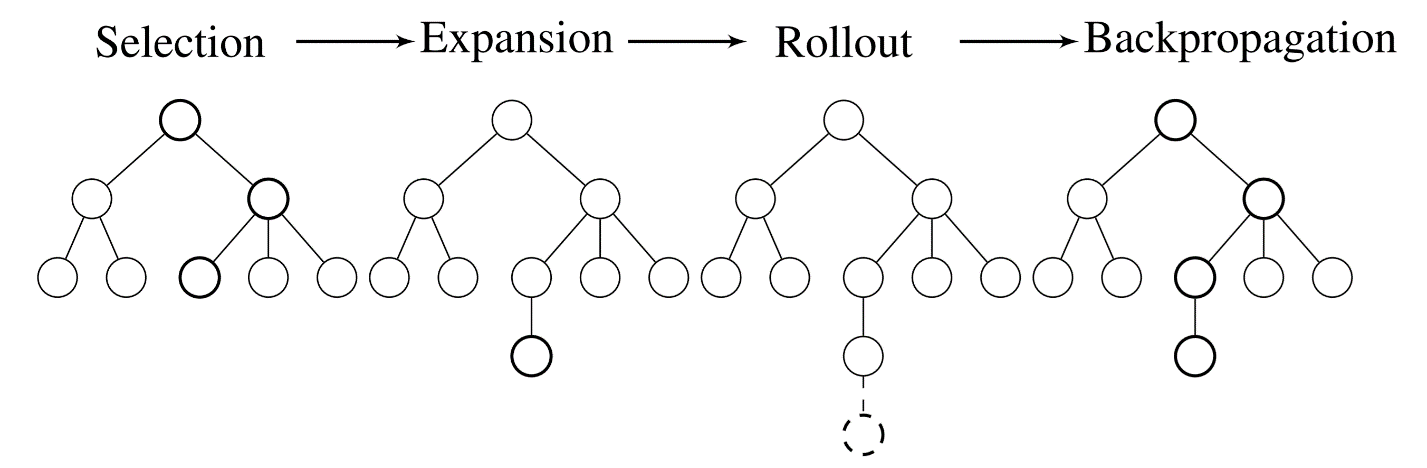
\includegraphics[scale=.825]{figures/MCTS}
\end{figure}


MCTS shares a problem in common with other RL algorithms. In reward-sparse state spaces it requires many samples to converge to an optimal policy. Also in complex domains where cyclic or aimless behavior is possible, we may not encounter any high valued node during our rollouts and therefore we will be unable to appropriately update the tree statistics. This problem is common when we use purely random rollouts because the action space may be dominated by one particular action type (in the case of Cluedo, move actions). Dobre addressed this issue in the domain of Settlers of Catan by the sharing of results via transpositions, sampling of action types and the use of afterstates \cite{Mihai}. A useful contribution of the prior literature is the use of action types instead of finer grained actions in the Monte Carlo tree. This hierarchical approach is necessary for two reasons: it simplifies the branching factor, and accounts for any differences between the cardinality of different action types. For example, the end turn action type has only cardinality of one, yet the action type move has a cardinality equal to the number of combinations of legal moves within the dice roll limit. This leads to an imbalance in our agent sampling more move actions over the action of ending the turn. While this may not be such an issue in the game of Cluedo where the action space is rather limited, it certainly is for games where many consecutive actions are possible. In fact, it is never optimal to end your turn in Cluedo if there is still a possible action to be taken. So we abstracted the action space further by removing ‘end turn’ as an action and we instead automatically end the turn when the player has no more possible actions to take. Afterstates, or sometimes known as successor-states, is a method for combining results of actions that lead to the same resultant outcome state. This is a huge benefit in Settlers of Catan due to the ability to abstract the game state in a way that many actions share outcomes. However, in Cluedo this effect is somewhat diminished due to the fact that our state representation must include the actual locations of the pieces (whereas there are no pieces in Settlers of Catan). This forces actions to have generally non-overlapping outcome states. However, due to time limitations we did not explore this further and leave it to future work. Consequently, our MCTS agent makes use of afterstates in the same fashion as Dobre.

Dobre improves the issues incurred by random sampling via introducing prior knowledge into the tree and rollout phases respectively. Due to time constraints, we were unable to collect such samples and therefore turned instead to a heuristic biasing approach. During both the tree and rollout phases, our MCTS agent plays against three Heuristic based agents who effectively bias the search into more fruitful areas of the tree. This also inhibits cyclic or ineffectual behavior as the agent must quickly learn how to find reward signals or it will rapidly lose against the informed agents.

After constructing this consistent tree, we simply need to select the action with the highest quality estimate to act optimally. However, because the algorithm is ‘anytime’ (meaning it can return estimates even if stopped early), stopping the algorithm before convergence can lead to suboptimal estimates and thus imperfect policies \cite{Gelly}. Therefore, choosing the action of maximum quality may lead us to play sub optimally, because that action has been estimated to have better quality than it really has. Or other actions with underestimated values are actually better. This ‘anytime’ property is very useful and while the estimates may be suboptimal for many nodes, nodes local to the root node (the current state) will be sampled enough to give us practical and valuable estimates. By biasing the search in favor of the highest valued nodes we can reduce the number of samples required to get reasonable estimates. The study of how to decide between n actions is explored using multi-armed bandit problems \cite{Gelly}. 

\section{Multi-armed Bandits}
A multi-armed bandit problem is a sequential decision problem over a set of possible actions ("arms") \cite{robbins1952}. At each time step, the player pulls one of the arms and recieves a pre-allocated and observable reward. The goal is to maximize the rewards obtained over a sequence of allocations and actions. The term multi-armed bandit comes from the sequential decision problem of playing multiple slot machines at once (the slot machines being the “multi-armed bandit”), and repeatedly choosing which arm to pull next. The player must balance the exploitation of arms that did well in the past and the exploration of arms that are currently underestimated but which may give higher payoffs in the future. 
When playing board games using reinforcement learning, each decision is made by simulating and evaluating as many possible game rollouts from the current state as time and resources allow. Algorithms for bandits (more specifically, for a tree-based version of the bandit problem) can be used to explore more efficiently the huge tree built by simulating game rollouts by focusing on the most promising subtrees (i.e. where the sampled return was greatest). A crucial algorithm in the literature, the UCT algorithm for hierarchical bandits of Kocsis and Szepesvari, which can be seen as an extenion of the UCB bandit algorithm, is directly applicable to these tree-based searches \cite{Kocsis2006}. UCT has demonstrable improvements over prior methods such as \(\epsilon\)-greedy, where the optimal action is selected with probability 1-\(\epsilon\) and a uniformly random action with the remaining probability \(\epsilon\). UCT is proven to converge to optimal and consistent decisions as the number of samples grows to infinity \cite{Kocsis2006}. The main idea is to bias the MCTS to bias search towards actions which have been tried he least number of times and therefore are the most uncertain \cite{Gelly}. This is an extension to the natural idea that one must balance between exploration (trying new actions) and exploitation (selecting the action of highest quality). These improvements stem from analyzing the regret of a player who pulls the arms according to some strategy. We can make comparisons between this strategy's performance with that of an optimal strategy that, for any n step horizon, consistently plays the best arm. Stated more simply, we analyze the regret of a player who does not always play optimally. This regret is typically formulated as follows:

\begin{equation}
R_n \defeq \max_{i=1,...,K} \sum_{t=1}^n X_{i,t} - \sum_{t=1}^n X_{I_t,t}
\end{equation}

Where we have K \(\geq\) 2 arms and sequences of rewards \(X_{i,1},X_{i,2}...\) associated with each arm \( i = 1,...,K\). Where at each time step \( t=1,...,N\) the player selects an arm \(I_t\) and recieves the pre-allocated reward \(X_{I_t,t}\).

The successes of UCB, and in turn the UCT algorithm, come from bounding this regret defined above. The UCT algorithm effectively moderates the tradeoff between exploitation and exploration by introducing a bias term which quantifies our uncertainty on the current estimates of the action values. UCT biases the value function with a confidence term that encourages actions to be explored fairly based on their estimates and the number of times they have been visited (not uniformly). This calculation is represented by the following equation:
\begin{equation}
UCT(s,a) = Q(s,a) + C \sqrt{\frac{2lnN(s)}{N(s,a)}}
\end{equation}
Where N(s) is the number of times the current state s has been visited, and N(s,a) is the number of times action a has been taken from state s. \\
Though multi-armed bandits have been studied in a plethora of environments we are mainly interested in the stochastic and Markovian settings. These settings apply most directly to tree search and thus planning over actions in complex games. This tree search is a sequential decision problem over states in a finite MDP. Like with multi-armed bandits, the assumptions are that the reward and transition distributions are unknown, and we want to act in the MDP so as to maximize the rewards. Another model, with many applications, is that of sleeping bandits. There, it is assumed that the available actions vary over time \cite{regretAnalysis}. Another interesting result is that of Kearns et al. who showed that regardless of the size of the state-space, fixed size trees suffice to find an action at the initial state whose value is within some error \(\epsilon\) of the best action \cite{Kearns2002}.

\section{Markov Decision Processes}
Reinforcement learning agents plan to maximize future cumulative return. If we try to define what this means mathematically we get the following sequence of rewards starting from any time step t:
\begin{equation}
R_t = r_{t+1} + r_{t+2} + r_{t+3} + r_{t+4}\ldots = \sum_{k=0}^\infty r_{t+k+1}
\end{equation}
If this sequence were to be infinite or we simply wish to tune how much we care about reward now rather than later it is commonplace to add a discount factor \(\gamma\):
\begin{equation}
R_t = r_{t+1} + \gamma r_{t+2} + \gamma^2 r_{t+3} + \gamma^3 r_{t+4}\ldots = \sum_{k=0}^\infty \gamma^k r_{t+k+1}
\end{equation}
Where \(0 \leq \gamma \leq 1\), with \(\gamma\) = 0 being a myopic agent to \(\gamma\) = 1 being a prudent one. Through interaction with the environment and the observation of these reward signals, the agent tries to maximize a function over the expected rewards. The end goal being to learn a policy that makes optimal decisions. A policy \(\pi\) being a mapping from every state \(s\) to a probability distribution over the action space \(P(A)\) for all \(a\in A\), with the probabilities being indirect measures of the value of each action \(a\) in state \(s\). 
To formalize the agent, its interactions with the environment, and the rewards it receives we can model it as a Markov Decision Process (MDP). A MDP is a sequential learning task that satisfies the Markov property: the next state and expected reward are dependent only on the current state and the action chosen and not on anything that preceded them (Russell and Norvig, 2009). In other words, the future is independent of the past given the present. Mathematically it means we assume the following factorization:
\begin{equation}
P(s_1, r_1, a_1 \ldots , s_t, r_t, a_t, s_{t+1}, r_{t+1}) = P(s_t, r_t | s_1, r_1, a_1 \ldots , s_{t-1}, r_{t-1}, a_{t-1}) P(s_{t+1}, r_{t+1} | s_t, r_t, a_t)
\end{equation}
Assuming that our process is markovian, we can go on to define the transition and reward probabilities. We define an MDP as a tuple \(<S,A,\mathcal{P},\mathcal{R}>\) of states \(S\), actions \(A\), the transition probabilities \(\mathcal{P}\), and the reward probabilities \(\mathcal{R}\). Where:
\begin{equation}
\mathcal{P}_{s{s^\prime}}^a = Pr(s_{t+1} = {s^\prime} | s_t = s, a_t = a)
\end{equation}
\begin{equation}
\mathcal{R}_{s{s^\prime}}^a = \mathbb{E}[r_{t+1} | s_t = s, s_{t+1} = {s^\prime}, a_t = a]
\end{equation}
Given the above definitions, the Bellman optimality equation (using action value notation) for an MDP is:
\begin{equation}
Q^*(s,a) = \sum_{s^\prime} \mathcal{P}_{s{s^\prime}}^a (\mathcal{R}_{s{s^\prime}}^a + \gamma \max_{a^\prime} Q^*({s^\prime}, {a^\prime}))
\end{equation}
The key here is that we can express values of states in terms of the values of other states. This allows us to 'bootstrap' estimates of our current state's value given estimates of the values of other states in the future. 

\section{Partially-observable Markov Decision Processes}
\subsection{Definition}
The full state of the real world is not fully observable, and many times the environments we wish our AI to function in are not either. This leads to a breakdown of the methods that use the MDP framework we just defined above. This is because the state transitions no longer have the Markov property. For example, when standing in a room, one is limited to their own perspective and may not be able to see objects which are occluded by others, objects in another room nor see behind themselves. This leads to an incomplete description of state, where we receive observations when we interact with our environment rather than the full state. Under these circumstances, MDP based methods make strong and unrealistic assumptions that will clearly lead to suboptimal policies. We would like to formulate a new framework under which we can reason about this hidden information and still make use of the highly rigorous MDP structure. To do this, we change the formulation of the problem, where we receive observations instead of full state descriptions and we leave rewards as a deterministic function of the observations. To incorporate these observations over time into our agent’s reasoning, it is natural to keep track of an agent’s history (or equivalent summary belief) over the course of its’ interaction with the environment. The concept of a belief seems like a natural component of the game Cluedo when you consider that the only partially observable information is the other players’ hands and the contents of the envelope. Thus, the entirety of this partially observable info can be captured in the player’s belief about those factors. Belief can be seen as a more compact and less unwieldy form of the history. We can incorporate these elements into the well-defined framework of Partially-Observable MDPs, or POMDPs. Sutton and Barto give a great compact summary of how a belief or history can be incorporated into the MDP framework:
\begin{quote}
In this approach the environment is assumed to have a latent state \(X_t\) that underlies and produces the environment’s observations, but is never available to the agent (and is not to be confused with the observable state used by the agent to make predictions and decisions). The natural Markov state, \(S_t\), for a POMDP is the distribution over the latent states given the history, called the belief state \cite{Sutton-barto}.
\end{quote}
More formally, we define a POMDP by extending an MDP to have a set of observations \(\Omega\) and defining the probability of observing an observation \(o \in \Omega\) given action a is executed and the resultant state is \(s^\prime\). An equivalent formulation is a Belief MDP which is defined as the tuple \(<B,A,\tau,\rho,\gamma>\) defined over a continuous belief state space \(b\in B\) where \(b\) is a probability distribution over all possible states \(s\in S\), \(A\) is the set of actions, \(\tau\) is the belief transition function \(\tau(b^\prime,a,b)\), and the reward function is \(\rho (b)\).
\begin{equation}
\tau(b^\prime,a,b) = P(b^\prime|b,a) = \sum_o P(b^\prime|a,b,o)P(o|a,b)
\end{equation}
\begin{equation}
\rho(b) = \sum_s b(s)R(s)
\end{equation}

\subsection{Methods for POMDPs}
For complex partially observable environments, exact methods like dynamic programming are unfeasible due to Bellman’s curse of dimensionality \cite{Mihai}. Instead most approaches use sampling or use an abstracted representation of the belief to plan (via factoring) \cite{Silver-veness} \cite{Kaebling-Lozano}. 
We can divide the most popular POMDP algorithms into three classes: sampling of determinizations, information sets, and belief states. Simply put, determinizations are the process of sampling fully observable states that are possible given the history of the game (belief) and performing Monte Carlo Tree Search on these samples of perfect information. However, this has two major weaknesses pointed out by (Cowling et. al, 2012): strategy fusion and duplication of work \cite{Cowling}. 
\begin{description}

\item \textbf{Strategy fusion:} The algorithm makes the flawed assumption that the same decisions can be made across determinizations, though this is demonstrably false, and as such leads to the fusion of different strategies from each determinization.
\item \textbf{Duplication of work:} Many of the determinizations will share common nodes, yet this is not exploited, and so work is duplicated across samples.

\end{description}

In an attempt to sidestep these problems, (Cowling et. al, 2012) developed an MCTS algorithm that operated on information sets of states instead of sampled determinizations \cite{Cowling}. This information set approach avoids the duplication problem by keeping track of all possible true states in one tree, however, strategy fusion is still an issue because the rollouts are still sampled via determinizations of the information set. To address this weakness, they proposed a new UCT rule that takes into account the number of times the action was legal in any given determinization. Further, they proposed an extension to ISMCTS to account for the beliefs of the other agents with multiple observer ISMCTS (MO-ISMCTS). However, this increases computational complexity because of the need to store and reason over multiple information set trees. While this is not of particular salience to Settlers of Catan (Dobre, 2018), in the game of Cluedo it is highly strategic to act in correspondence with the belief states of other agents \cite{Mihai}. This can be demonstrated by considering which cards you wish to suggest, taking into account that bluffing is a profitable strategy under certain circumstances, or which cards have been shown to a suggester by a third agent. As mentioned previously, this dissertation is highly influenced by the work of (Silver and Veness, 2010) on planning in large POMDPs, and the thesis of (Dobre, 2018) which explores low-resource learning in complex games \cite{Silver-veness} \cite{Mihai}. Both of these papers explore planning in the belief state space, which is conceptually very similar to that of information sets. Belief states can be represented by particle filters (Silver and Veness, 2010), factored representations (Dobre, 2018) and though not explored here, hidden markov models/ Dynamic Bayesian networks (Russell and Norvig 2009) \cite{Silver-veness} \cite{Mihai} \cite{Russell-norvig}. POMCP and ISMCTS both sample a fully observable state from the current belief state, then mask out the illegal (impossible) parts of the tree \cite{Mihai}. The number of samples required by these algorithms scales with the support of the belief distribution and its entropy. Because they work with determinizations, both algorithms effectively consist of two sampling phases, one to estimate the current belief and one to estimate the expected return for each sample. This is disadvantageous and incurs increased computational complexity. In contrast, BMCTS does not sample fully observable, but rather propagates the belief in the tree stage and approaches the problem of strategy fusion in the same way as ISMCTS; by modifying the UCT calculations to account for action legality. Dobre’s algorithm plans in an almost exact representation of the belief by making use of a factored representation \cite{Mihai}. The propagation of belief however requires additional computational load. In an effort to see if this extra complexity was warranted, Dobre experimented with sampling fully observable states at leaf nodes and performing rollouts just like POMCP and ISMCTS; this agent is called, BMCTS with Observable Rollouts (BMCTSOR). It turned out that this agent which worked with observable rollouts outperformed the agent which planned entirely in the belief space. We follow Dobre in using the standard POMDP framework to present the algorithms. However, we do not make the assumption that the opponents have the same strategy as our own agent, i.e. self-play. Instead our opponents are modelled using a factored version of the Heuristic agent we present later.

\section{Parallel MCTS}
The following section is based off of Mihai Dobre’s PhD thesis, because we directly make use of his parallelized MCTS code. MCTS is a straightforward algorithm to parallelize. This is necessary due to the time constraints of this dissertation, and the need to effectively sample within a reasonable time limit. There are three options to parallelize the algorithm, using leaf parallelization, root parallelization or tree parallelization \cite{Mihai}. Leaf parallelization parallelizes the rollout phase and then backpropogates the final results through the tree once all threads have halted. Dobre claims that it is the simplest of the three algorithms but comes with a few drawbacks. To begin, since it is necessary to wait for all threads to finish their respective rollouts, it is inefficient when it comes to backpropagating results. There is also an ambiguity with updating the UCT values when the node visits are incremented in steps greater than 1. On the other hand, root parallelization makes a copy of the game tree for each thread. After all threads have finished, the results are combined and the next decision can be made. Mihai claims that it “generally performs better than leaf parallelisation, but it requires a good combination of the final results” \cite{Mihai}. Because this requires a copy of the game tree per thread, it is highly memory inefficient. Tree parallelization avoids this issue by making use of locks and takes a more typical parallelized approach. Dobre’s implementation uses local locks, where the local part of the tree is locked when a thread accesses it. In an effort to reduce overhead, Dobre also made use of ‘virtual loss’, which discourages similar trajectories by multiple threads.

\section{Domain Analysis}
Cluedo is a complex, non-cooperative game of imperfect information where turns are taken sequentially and the goal of the game is symmetric; to reduce the entropy about the contents of the envelope enough to accurately accuse the correct weapon / suspect / room tuple. The game is also non-deterministic, following from stochasticity inherent in the dice rolls. The imperfect information comes into play when a player observes (but is not a participant in) a suggestion and a succeeding falsification of said suggestion. Inductively reasoning about these observations are of high strategic importance for an optimal Cluedo agent yet are also not a necessity for winning. Unless you assume all the other agents are optimal inductive reasoners, in which case a lucky accusation is the only avenue to win in the absence of information gathering from the aforementioned observations. This is because the goal of the game can be abstracted from correctly accusing, to a race to reduce entropy. This follows from the fact that reducing entropy to zero effectively means that you know the location of every card. Subsequently, any information which can lead to a reduction in entropy about the contents of the envelope must be taken advantage of. This includes the content of suggestions, which can inform a player about the suggester’s hand/intentions, if you reason about player types. Computation becomes increasingly expensive as the model reasons over nested beliefs and different player types. Due to time restrictions, we leave the avenue of reasoning over player types (and thus induction about the contents of a suggestion) to future work. 

Even more information however can be gleaned from the observation of who falsified the suggestion in conjunction with the content of the suggestion. If a suggestion has been falsified by another agent, it can be said with absolute certainty that said agent has one of the three cards suggested. If through keeping track of our belief of where all cards are, we already know that two of the cards are accounted for (and not in the hand of the falsifier), we can deduce that the falsifier’s hand contains the final card. On the other hand, if only one or none of the cards are accounted for then we can still update our beliefs via a Bayesian update given the probabilities of an observation and the probability of the observation given the pmf of each suggested card. This improvement indeed saw increased performance for our heuristic agent compared to the same agent who does not reason over partially observable interactions. Choosing which cards to suggest too has strategic importance, as mentioned before other players can reason about your hand based off of your suggestions. Since we deferred to address this type of reasoning, we here also defer strategically suggesting in order to avoid revealing information or misleading other players about the agent’s hand. Instead, our most advanced agent simply suggests the tuple with highest entropy. 

Taking a turn in Cluedo is where the complexity of the game creeps in due to turns consisting of one or two actions respectively. At the same time however, the game rules lend themselves to a natural hierarchy of action-types over the action space and the action types are further subdivided into two distinct yet flexible main phases of a turn. At the beginning of each player’s turn the optimal play is to accuse if you have sufficient knowledge of the envelope or to move instead. A slight simplification we made to reduce action space complexity was to only allow accusations in this beginning phase as the alternative, to also allow an accusation after a move, is redundant because a move itself provides no information and thus the two sequences are equivalent in terms of belief. Per the rules an agent cannot suggest in this first stage of a turn unless in the intermediate play between turns, the character their token represents has been suggested and thus moved to the suggested room. The second phase of a turn is then conditional on two factors: the first phase action was a move, and that move left the player’s token in a room. If both conditions are met, a player may then suggest their current room and any weapon-suspect pair they choose. This regular structure in turn taking leads into predictable sequences of moves and suggestions until an agent is confident enough to accuse. None of our implemented heuristic agents accuse until the entropy of the envelope is zero. While a human may accuse earlier due to an overly optimistic strategy or based on some knowledge of their opponents’ player types and suggestion histories. 

\chapter{Description of work undertaken}
\section{CluedoSim}
\begin{figure}[h]
\caption{The CluedoSim environment (left: only heuristic agents, right: 3 heuristic agents and a human player)}
\centering
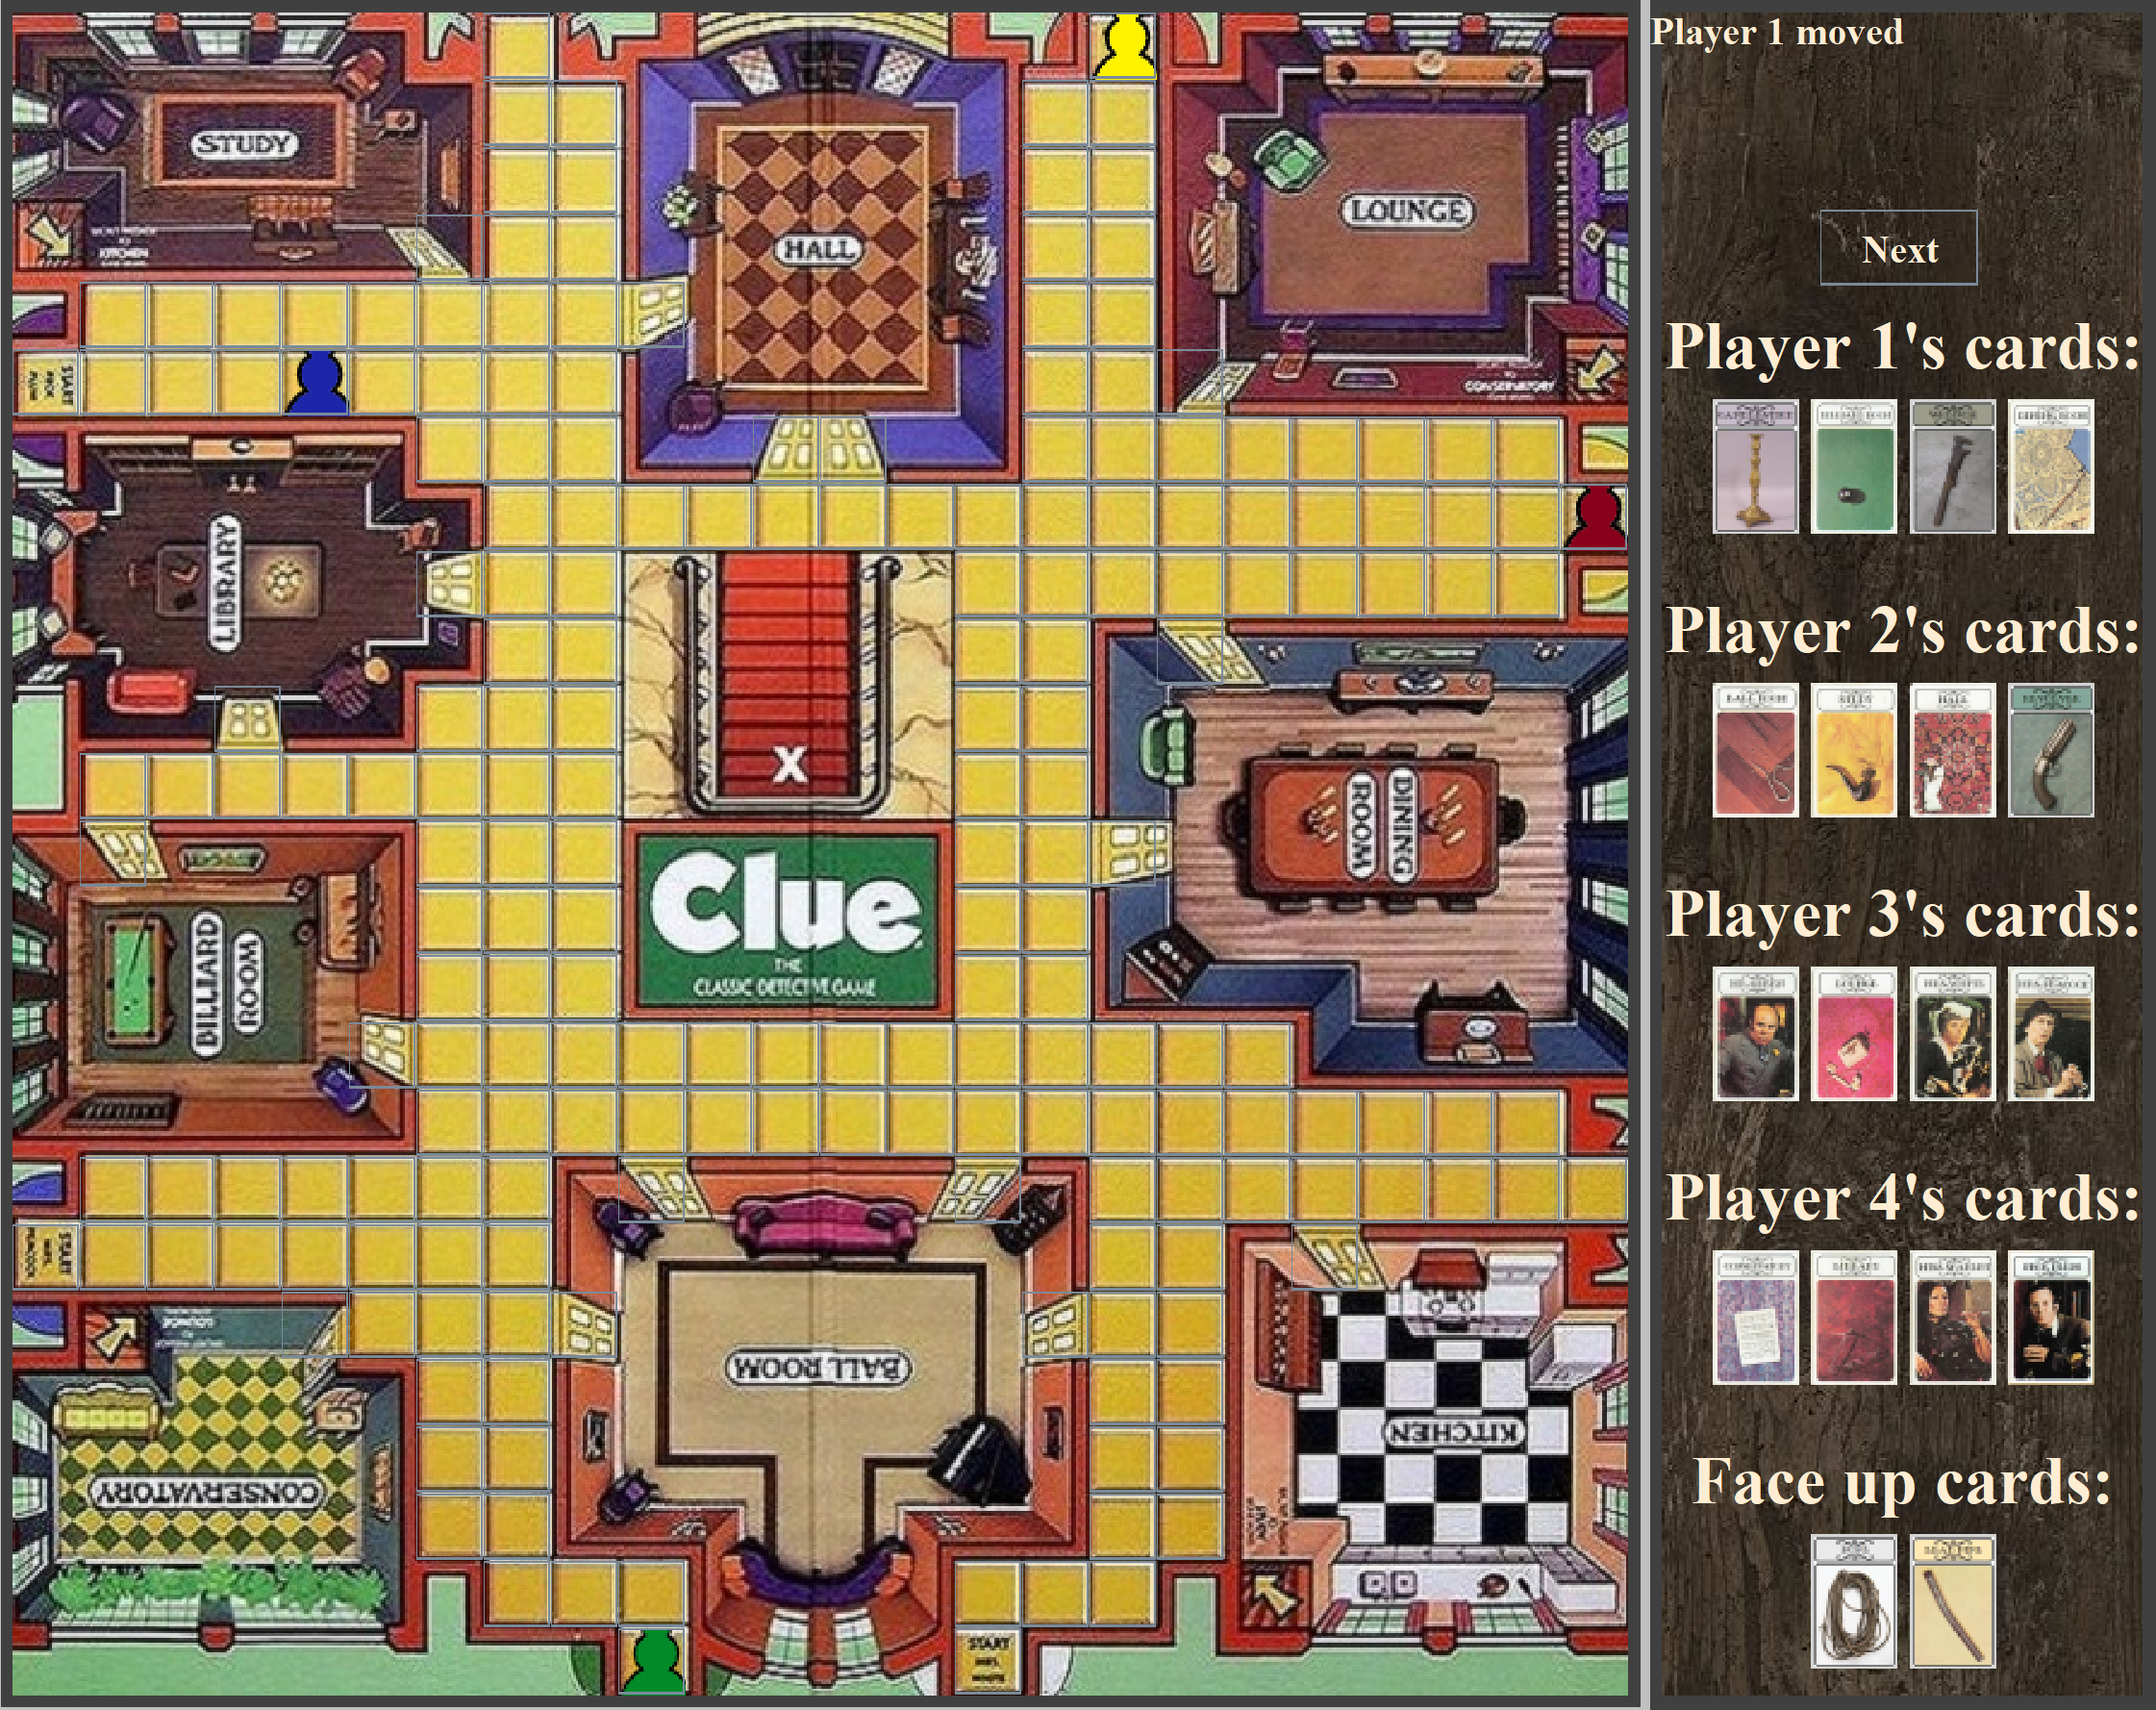
\includegraphics[scale=.3]{figures/cluedoSim}
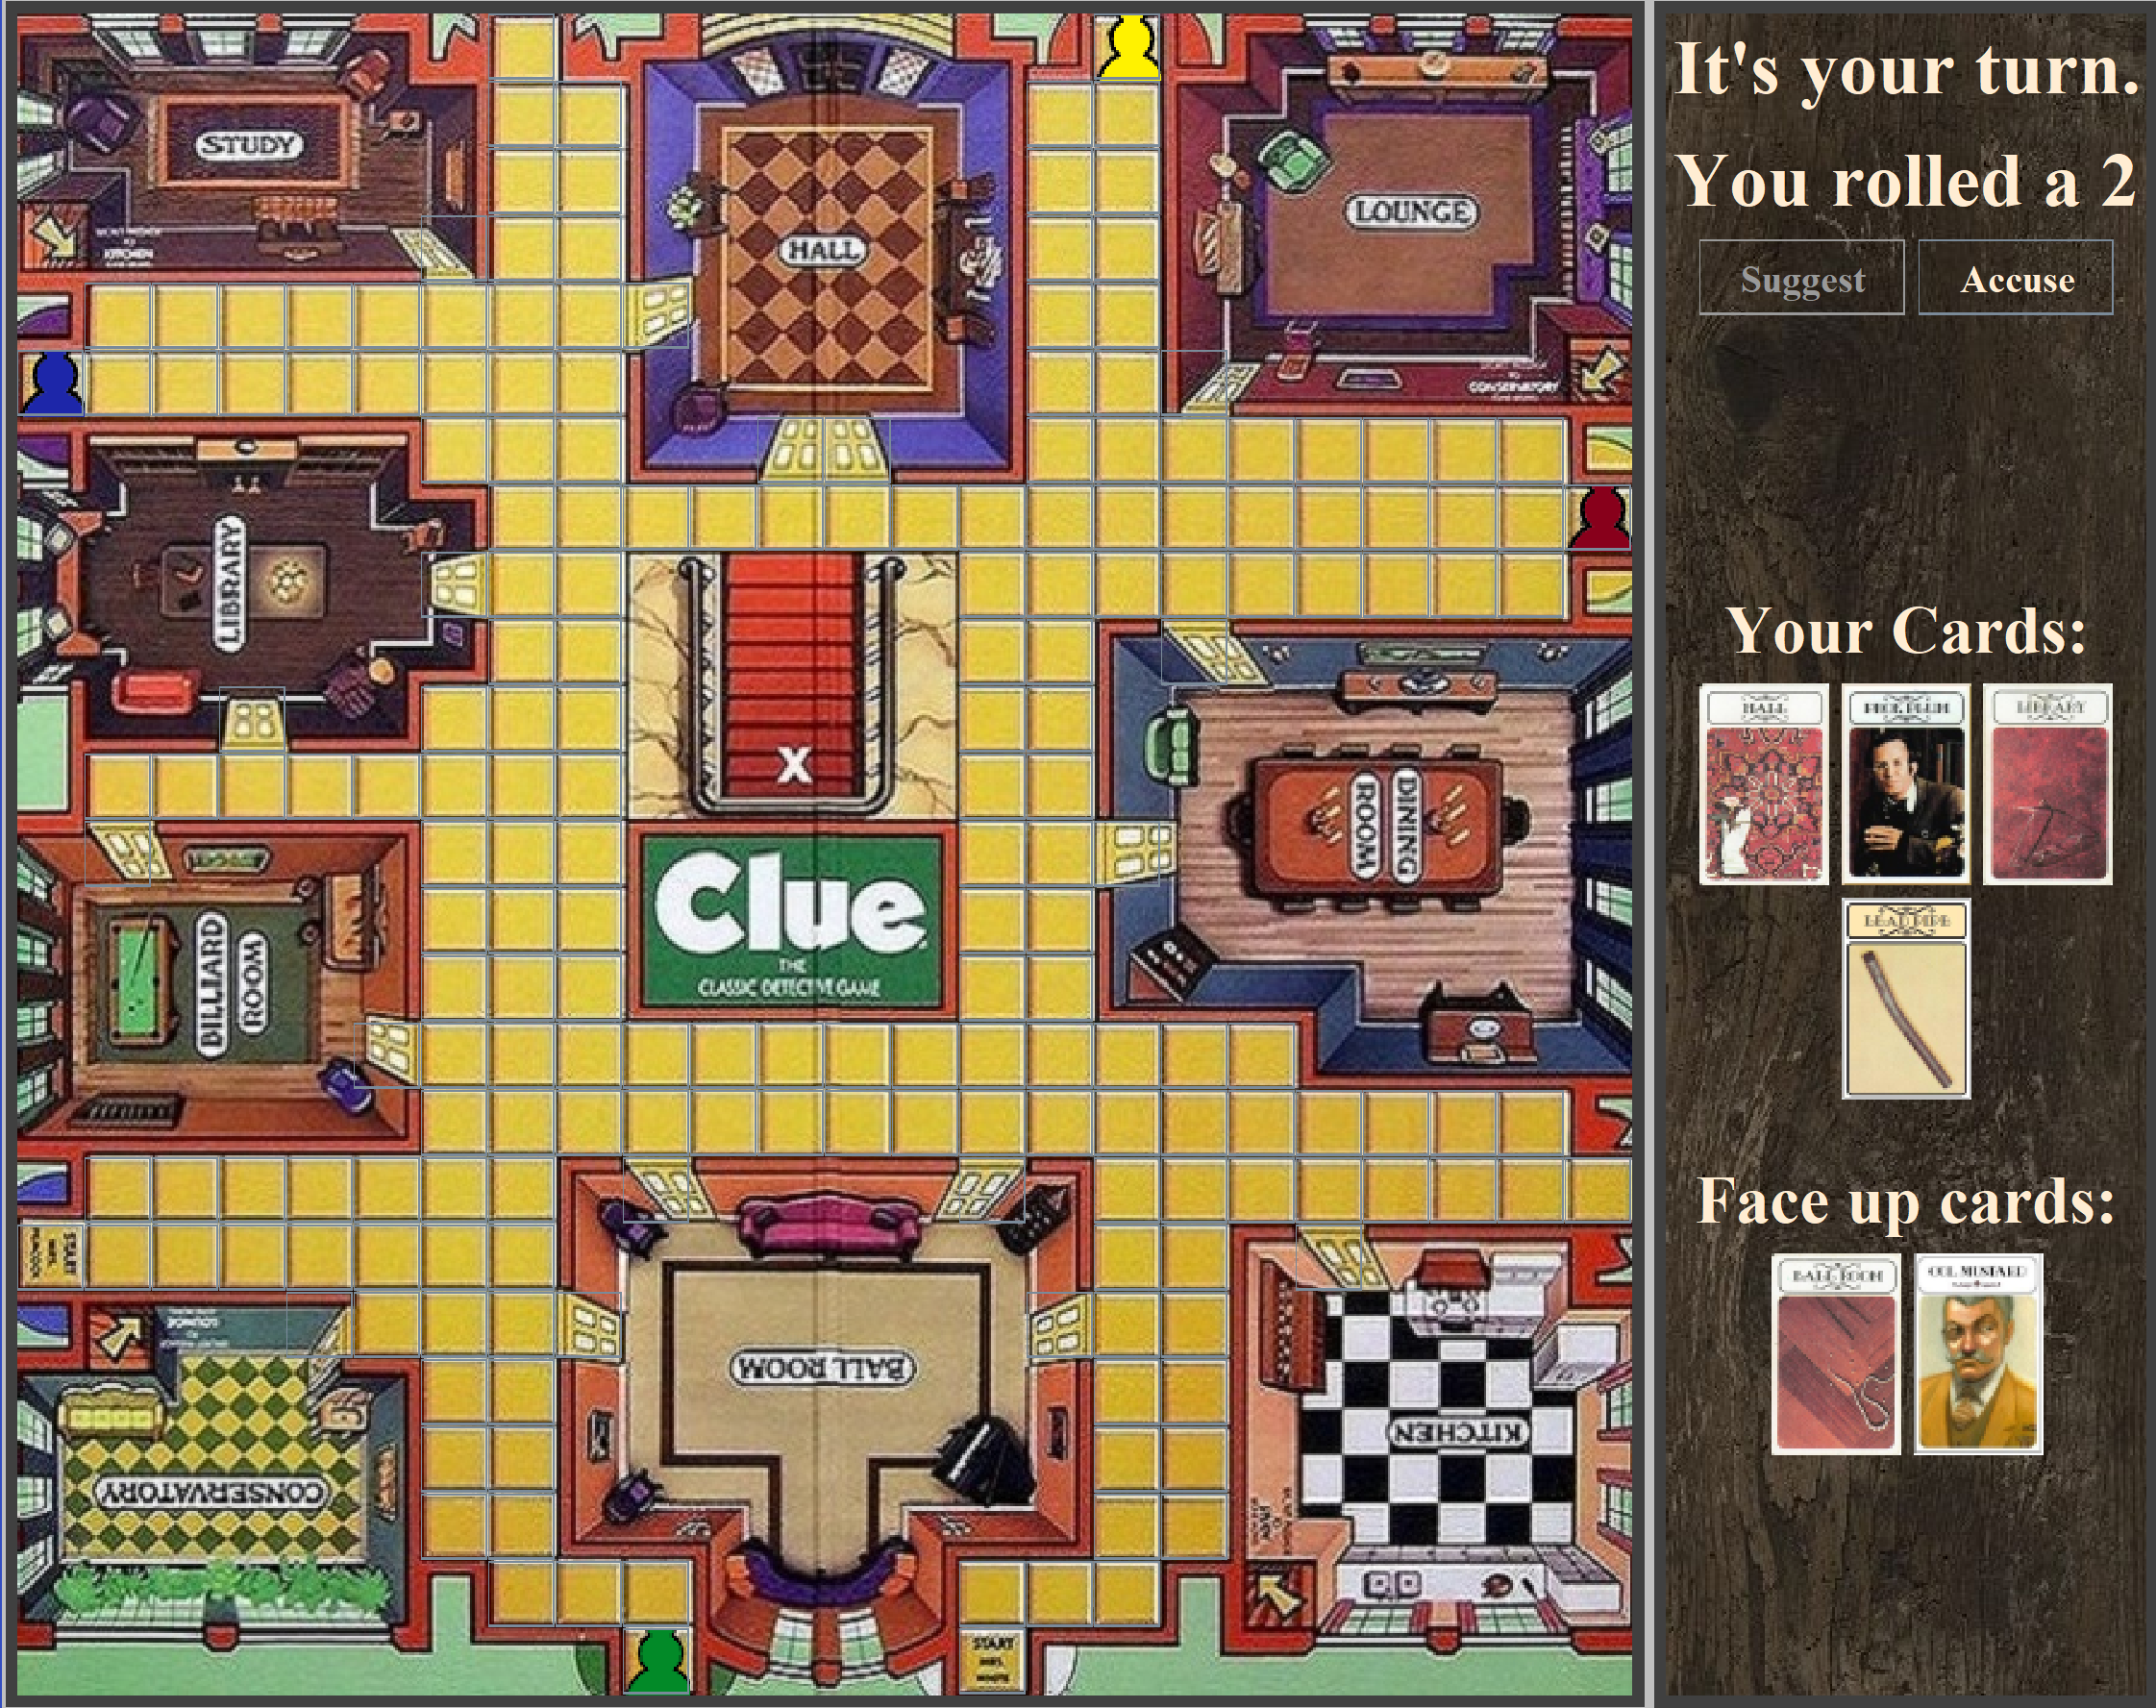
\includegraphics[scale=.3]{figures/humanCluedoSim}
\end{figure}

The first step was to build a simulator for the game with which we could test our agents against each other and time permitting, measure them against human performance. With this end in mind, and also for testing purposes, a GUI was necessary and was assembled using Java’s Swing package. The game logic and heuristic agents were also coded in Java and communicate via a player interface which allows for easy extension or implementation of new agents. It was also necessary to use a database to log game-specific info and also record the results of many games. This was achieved using MongoDB. 

\section{Heuristic agent}
The heuristic agent combines the AStar algorithm for path finding and an entropy centered heuristic for making suggestions. The agent always aims to suggest the room-weapon-suspect tuple with highest current entropy. Explicit probabilities for each card are kept and updated after observations from other agents (when any suggestion is proved false). These probabilities are represented as a 21x5 matrix, where the rows correspond to each card and the columns to the envelope (0) and the players 1-4. Therefore, entry 15,1 of the matrix tells us the probability that player 1 has the card whose index is 15, etc. When the observation is partially observable, i.e. when the agent is neither the suggester nor falsifier, the agent updates the card probabilities using Bayes rule.

\chapter{Evaluation and Analysis}

\chapter{Conclusion}

\appendix
\chapter{State Representation}
The following features were used to represent the states for the MCTS agent. The features used (in the order used in the state vector) were:

\begin{description}
\item \textbf{0:} The current game state. 0 if the game is still being played and 1 if the game has terminated.
\item \textbf{1:} The index of the current player
\item \textbf{2:} Boolean, if the current player has moved this turn
\item \textbf{3:} The room of the current player represented as the room's index (-1 if the player is not in a room)
\item \textbf{4:} The current roll (0 if the dice have not been rolled)
\item \textbf{5:} Whether or not the player is currently falsifiying a suggestion
\item \textbf{6:} Boolean, if the current player has suggested this turn
\item \textbf{7:} If this is a falsify state (feature 5), this is the suggested room index
\item \textbf{8:} Same as before. The suggested suspect index
\item \textbf{9:} Same as before. The suggested weapon index
\item \textbf{10:} Same as before. The index of the player who made the suggestion.
\item \textbf{11:} Boolean, if player one has accused.
\item \textbf{12:} Boolean, if player two has accused
\item \textbf{13:} Boolean, if player three has accused
\item \textbf{14:} Boolean, if player four has accused
\item \textbf{15:} The current entropy of the BMCTS agent
\item \textbf{16:} If the game state (feature 0) is 1, this is the winning player's index
\item \textbf{17:} The x coordinate of player one
\item \textbf{18:} The y coordinate of player one
\item \textbf{19:} The x coordinate of player two
\item \textbf{20:} The y coordinate of player two
\item \textbf{21:} The x coordinate of player three
\item \textbf{22:} The y coordinate of player three
\item \textbf{23:} The x coordinate of player four
\item \textbf{24:} The y coordinate of player four
\item \textbf{25:} If a player has accused and we are making a nature move to check if the player has won or lost
\item \textbf{26:} If a player has accused this is the index of the accused room
\item \textbf{27:} Same as before, this is the index of the accused suspect
\item \textbf{28:} Same as before, this is the index of the accused weapon
\end{description}

\chapter{Abstract Belief Representation}
The belief is represented as a twenty-one by five matrix where each row indexes a card and each column indexes the envelope and players. In this way each row is a probability mass function representing the probability of where that card is. Either in a player's hand (indices 1-5) or in the envelope (index 0). This belief representation is used by both the MCTS agent and the Heuristic agent. When initialized at the beginning of the game, a player's belief will have a total entropy of 30 (two face up cards and the four cards in the player's hand are known). All unkown cards start out with a pmf with probability equally distributed amongst the envelope and other players.

\newpage
\nocite{*}
\bibliography{references} 
\bibliographystyle{acm}

\end{document}
